\documentclass[]{article}

\usepackage{listings}
\usepackage{color}
\usepackage{amsmath}
\usepackage{graphicx}
\usepackage{float}
\usepackage[title]{appendix}
\usepackage[ansiapaper, portrait, margin=1.5in]{geometry}
\usepackage{hyperref}

\usepackage{caption}
\usepackage{subcaption}

\usepackage[backend=bibtex]{biblatex}
\addbibresource{comp-physics-project-may6.bib}

\definecolor{dkgreen}{rgb}{0,0.6,0}
\definecolor{gray}{rgb}{0.5,0.5,0.5}
\definecolor{mauve}{rgb}{0.58,0,0.82}




\hypersetup{
	colorlinks=false %set true if you want colored links
	linktoc=all,     %set to all if you want both sections and subsections linked
	linkcolor=blue,  %choose some color if you want links to stand out
}
\hypersetup{hidelinks}

\lstset{frame=tb,
	language=Python,
	aboveskip=3mm,
	belowskip=3mm,
	showstringspaces=false,
	columns=flexible,
	basicstyle={\small\ttfamily},
	numbers=none,
	numberstyle=\tiny\color{gray},
	keywordstyle=\color{blue},
	commentstyle=\color{dkgreen},
	stringstyle=\color{mauve},
	breaklines=true,
	breakatwhitespace=true,
	tabsize=3
}

%opening
\title{May 6th Weekly Report}
\author{Erik Bigwood}

\begin{document}

\maketitle

\begin{abstract}
Showing work completed up to May 6.
\end{abstract}

\tableofcontents
\newpage

\section{Harmonic Oscillator Demonstration}
\paragraph{Basic algorithm}
See the section "Algorithm improvements" for explanations of the actual code used here.

To begin, we define the problem setup -- $m$, $k$, $n$, and the bounds for $q$ and $\dot{q}$. For this demo, I've defined $(m_k) = (2,4)$ s.t. $k/m=2$. Define the Lagrangian function, and the methods QDD and QDDv to calculate $\ddot{q}$ at each $(q,\dot{q})$ point. Create $n$ point grids over $q$ and $\dot{q}$ and flatten those grids to $(n^2,1)$ arrays. Then, create a synthetic dataset with the given $(m,k)$ and store it.

\begin{figure}[H]
	\caption{$\ddot{q}$ vs. $(q,\dot{q})$}
	\centering
	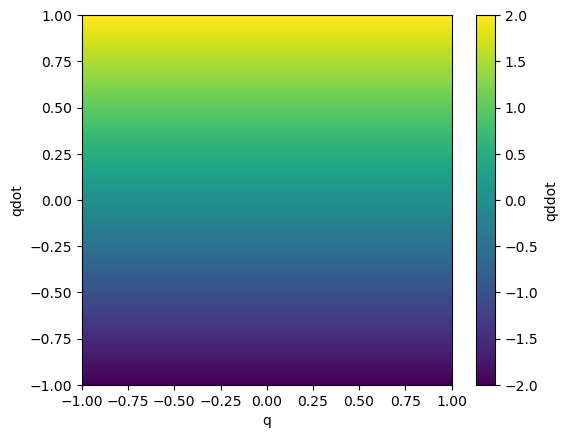
\includegraphics[scale=0.55]{qddot-vs-q-qdot.png}
	\label{fig:qddot-vs-q-qdot}
\end{figure}
Here I define the loss/error function as the summed $L^2$ norm of the difference between predicted and true data:
\begin{eqnarray}
	loss = \frac{1}{N}\sum_{i=1}^N \Big( \ddot{q}_{trial} - \ddot{q}_{true}\Big)^2
\end{eqnarray}

Now,disregard the specified $(m,k)$ values given in the problem setup and calculate the summed $L^2$ loss function for a grid of trial $(m_{trial},k_{trial})$ points. Due to the structure of this Lagrangian, the loss minimum is the line from the origin where $k_{trial}/m_{trial} = k/m$. The loss becomes extremely large as $m_{trial}$ becomes small, which will require some adjustment to the gradient descent algorithm later.

\begin{figure}[H]
	\caption{Loss landscape : $\frac{k}{m}=2$}
	\centering
	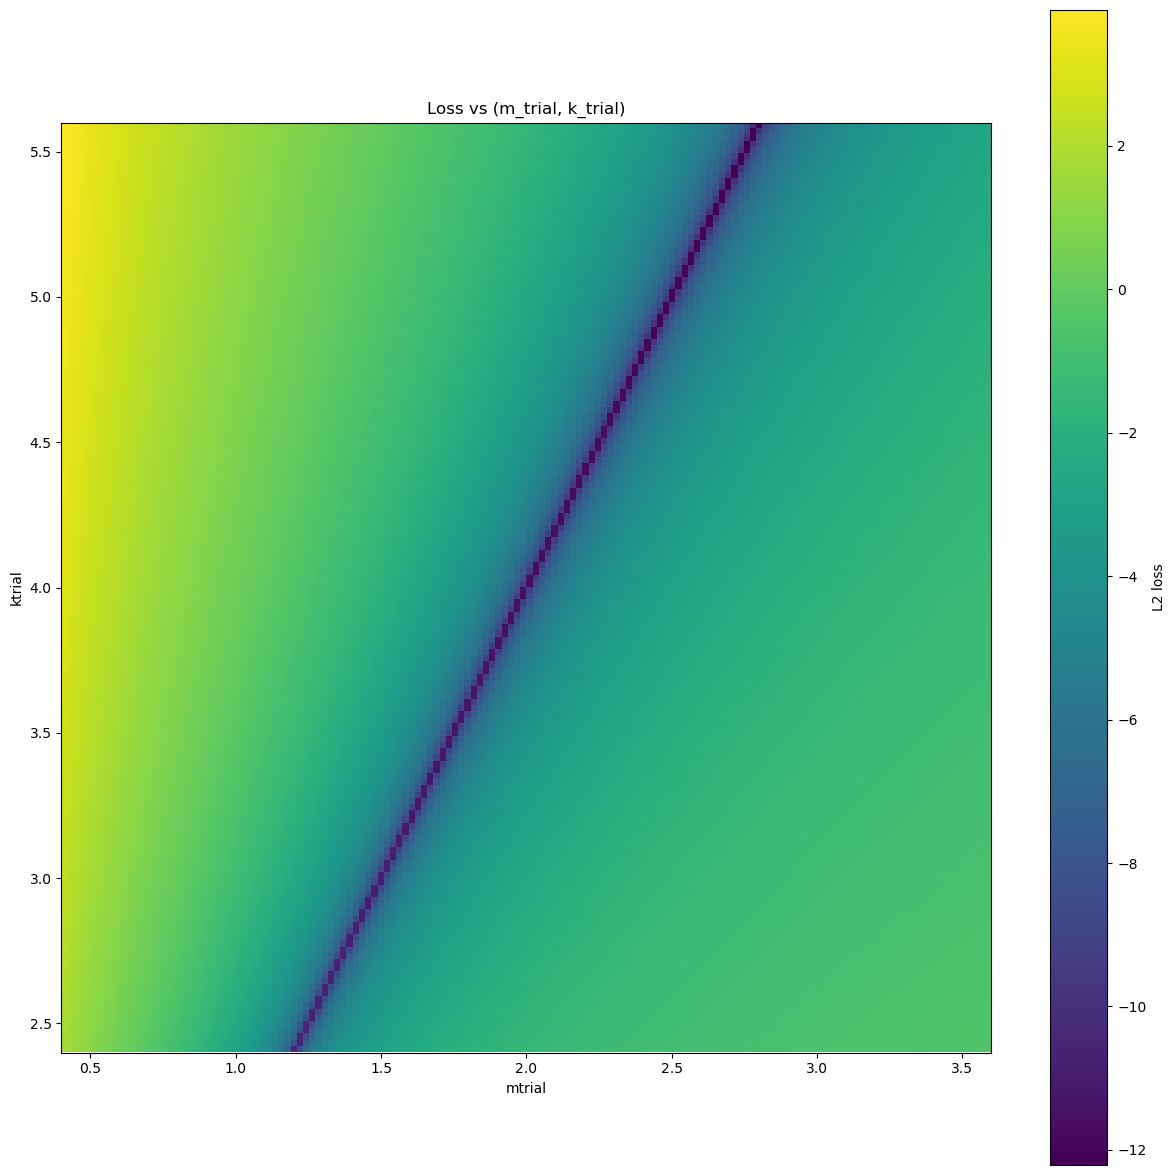
\includegraphics[scale=0.26]{loss-landscape.png}
	\label{fig:loss-landscape}
\end{figure}

As a simple demonstration, take a random $(m_{trial},k_{trial})$ point and perform gradient descent, shown in \ref{fig:parameter-fit}. The parameters $(m_{trial},k_{trial})$  converge to a solution with $k/m=2$ as expected, but due to the symmetry in the loss landscape, the actual values depend on the initial guess.

\begin{figure}[H]
	\caption{Gradient descent parameter fit : $\frac{k}{m}=2$}
	\centering
	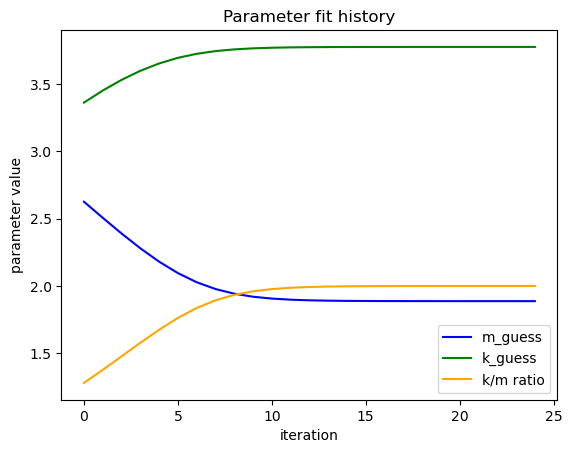
\includegraphics[scale=0.70]{parameter-fit.png}
	\label{fig:parameter-fit}
\end{figure}

Finally, Fig. \ref{fig:parameter-paths} contains a plot with the loss landscape and a series of parameter paths for a large number of random initial guesses of $(m_{trial},k_{trial})$. As mentioned earlier, the extreme range of loss values is compensated for by including a modification to the learning rate given by:
\begin{equation}
	\epsilon = \epsilon_0 e^{-\Big(\epsilon_0 \big| \nabla_{m,k} loss\big|\Big)^3}
\end{equation}

This reduces the effective learning rate when $|\nabla_{m,k} loss|$ becomes large, so that the parameters still evolve slowly enough to converge and not skip over the solution space.

\paragraph{Adding noise}
Adding noise to the synthetic dataset complicates the situation. In Fig. \ref{fig:loss-vs-noise}, I've included a plot comparing the loss function on a slice perpendicular to the solution space. On the left we have the unperturbed loss function, and on the right the loss function under a perturbation by normally distributed noise on each point in the $q,\dot{q}$ grids.

\begin{figure}[H]
	\caption{Loss vs noise on a slice perpendicular to the solution space}
	\centering
	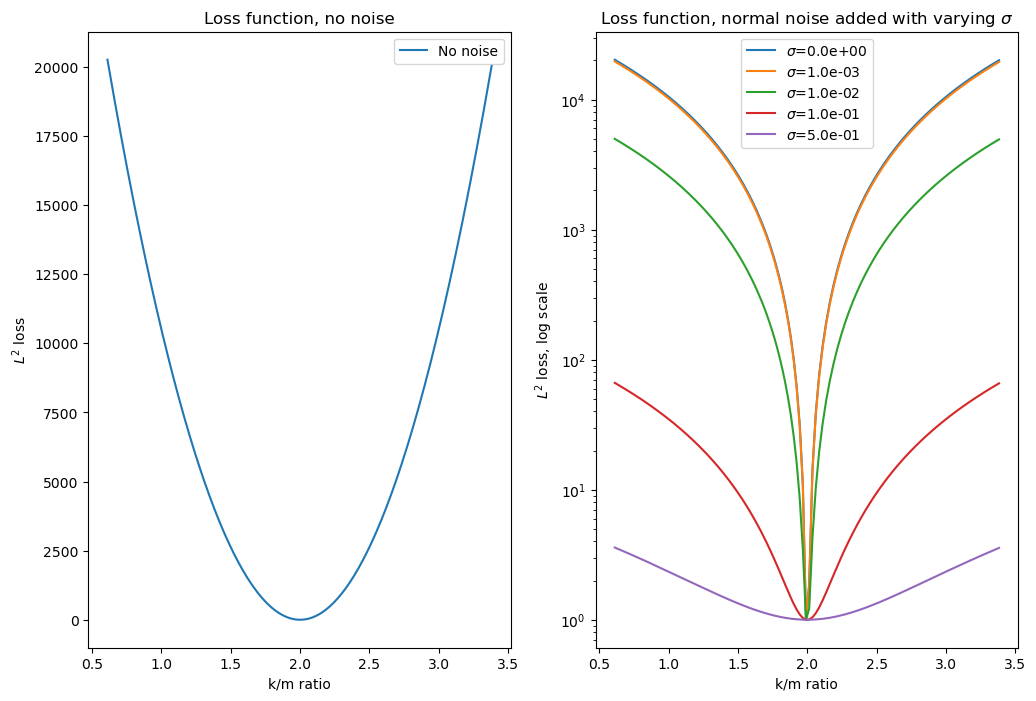
\includegraphics[scale=0.40]{loss-vs-noise.png}
	\label{fig:loss-vs-noise}
\end{figure}

Comparing the RMS error on the loss function caused by perturbation by noise (Fig. \ref{fig:rms-error-vs-sigma}) leads to a notable trend -- $\sigma\leq10^{-1}$ is effectively undetectable, but increasing noise intensity beyond that threshold leads to a dramatic increase in RMS error. More specifically, the loss function flattens out dramatically, washing out the nicely defined valley of low loss in the solution space. This demands more careful choice of the trial $(m_{trial},k_{trial})$ values and learning rate $\epsilon_0$. One potential approach is to evaluate the gradients at a large number of intial guesses and choose $\epsilon_0$ to restrict the gradient descent step size for the largest gradient sampled.



\begin{figure}[H]
	\caption{RMS error on loss vs. noise $\sigma$ on a slice perpendicular to the solution space}
	\centering
	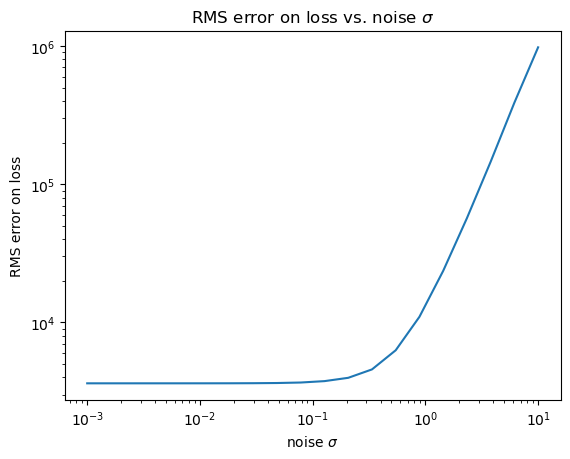
\includegraphics[scale=0.60]{rms-error-vs-sigma.png}
	\label{fig:rms-error-vs-sigma}
\end{figure}


In Fig. \ref{fig:loss_noise_no_noise}, I've included density plots of the loss landscapes with and without noise. Including noise broadens the valley of low loss and dramatically reduces the range of the loss function values, decreasing the gradients and slowing down convergence without compensating in the gradient descent algorithm.

\begin{figure}[H]
	\caption{Loss landscape with and without noise}
	\begin{subfigure}{.5\textwidth}
		\subcaption{Loss landscape, no noise}
		\centering
		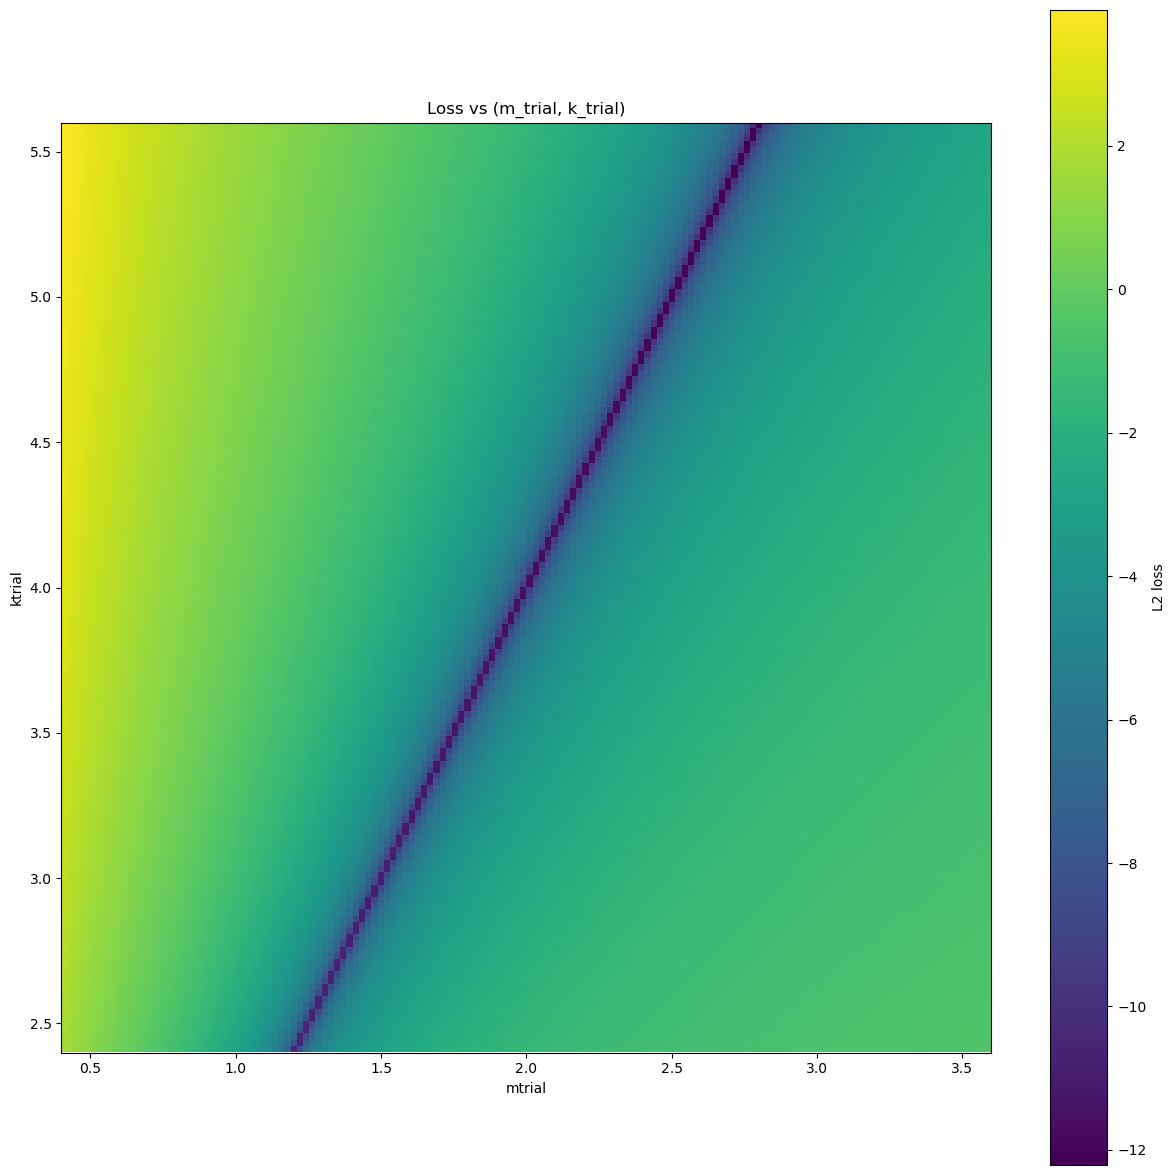
\includegraphics[scale=0.20]{loss-landscape.png}
		\label{subfig:loss-landscape}
	\end{subfigure}
	\begin{subfigure}{.5\textwidth}
		\subcaption{Loss landscape w/ noise, $\sigma=0.2$}
		\centering
		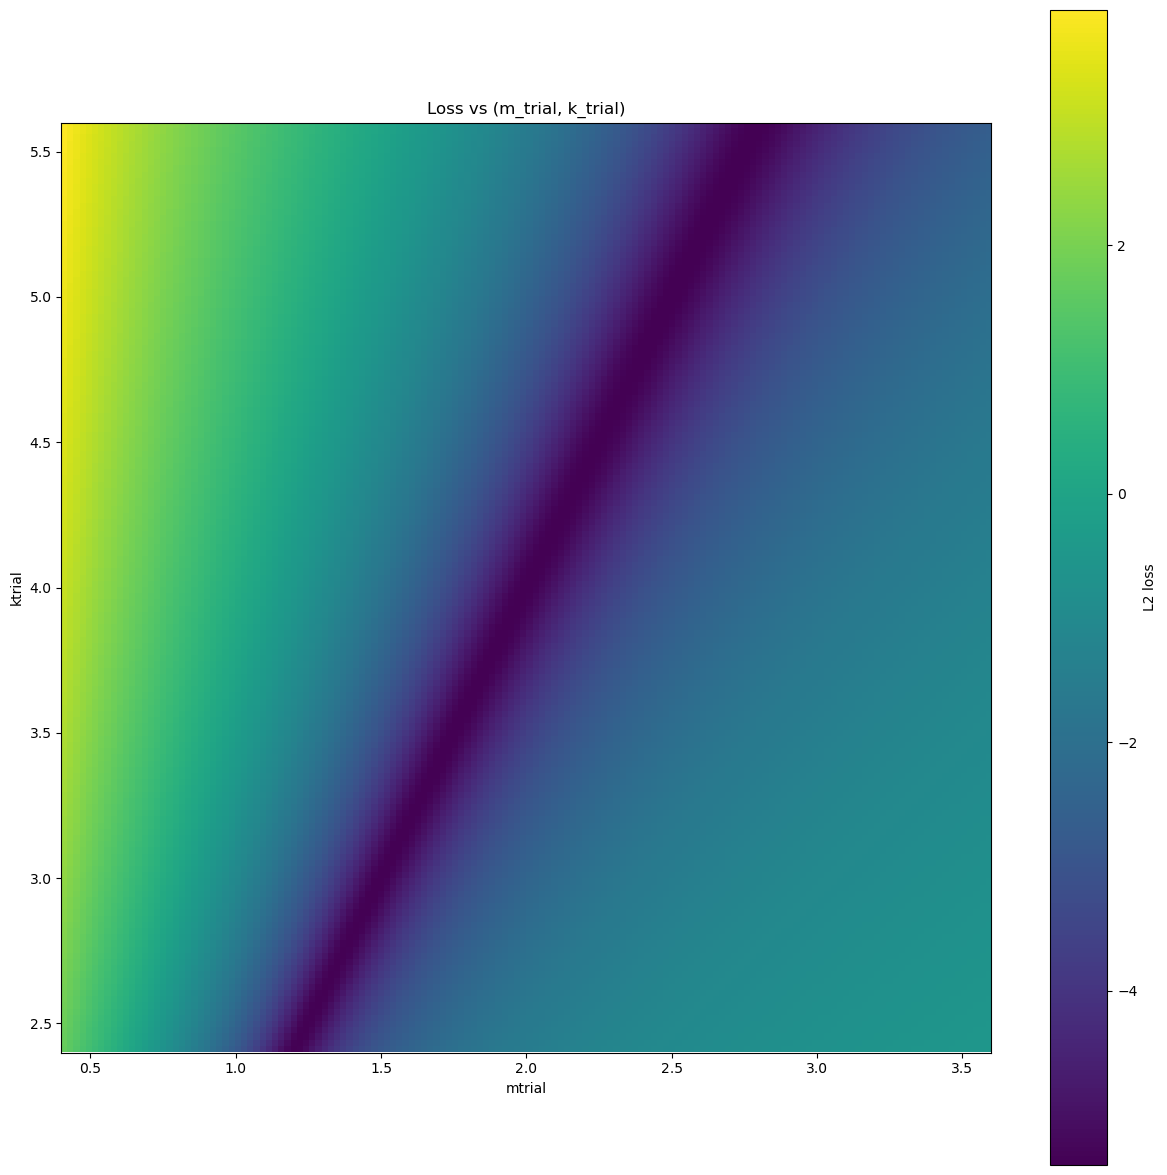
\includegraphics[scale=0.20]{loss-landscape-noisy.png}
		\label{subfig:loss-landscape-noisy}
	\end{subfigure}
	\label{fig:loss_noise_no_noise}
	
\end{figure}


\section{Algorithm improvements}

\subsection{Calculating $\ddot{q}$}
My previous work was based on using Pytorch\cite{Paszke2019}'s torch.autograd's Hessian and Jacobian to compute $\ddot{q}$ \cite{Cranmer2020}. Notably, these functions calculate $\textit{all}$ derivatives/2nd derivatives at all points, which can be a significant waste of compute. This week I've re-written the core code to utilize the torch.func module. This module includes torch.fun.jacfwd (Jacobian, forward-mode automatic differentiation) which I'm using to calculate derivatives, and torch.func.vmap which is an auto-vectorization method that wraps around a function and handles batching seamlessly. I suspect the torch.func methods are creating the computational graph in the background and tying everything together instead of re-creating it at each iteration.

My older method for calculating $\ddot{q}$ follows roughly this example (the indexing/linear algebra is simplified here by only considering a 1D harmonic oscillator\cite{Taylor2005}):
\begin{lstlisting}
def L(vec): #Harmonic oscillator Lagrangian density
	#input: array (m,k,q,qdot), returns Lagrangian density
	m, k, q, qdot = vec[0], vec[1], vec[2], vec[3]
	return 0.5*m*qdot**2 - 0.5*k*q**2
	
def qddot(Lag,m,k,q,qdot):
	#Returns d^2/dt^2 q given Lagrangian L
	v = torch.cat((m,k,q,qdot))
	full_hessian = autograd.functional.hessian(Lag,v)
	full_grad = autograd.functional.jacobian(Lag,v)
	
	grad_q = full_grad[2]
	hess_q = full_hessian[2,2]
	hess_qdot = full_hessian[3,3]
	hess_q_qdot = full_hessian[2,3]
	qdd = (hess_qdot**(-1))*( grad_q - hess_q_qdot*qdot )
	return qdd
	
m = tensor([1.])
k = tensor([2.])

out = torch.zeros(n_points**2) #out[i] = qdd(q[i], qdot[i])

#define q,qdot grids
qgrid = torch.linspace(q_min,q_max,n_points)
qdotgrid = torch.linspace(qdot_min,qdot_max,n_points)

for i in range(n_points): #iterate over q
	for j in range(n_points): #iterate over qdot
		q = tensor([qgrid[i]],requires_grad = True) #store iterated q
		qdot = tensor([qdotgrid[j]],requires_grad = True) #store iterated qdot
		qdd = qddot(L2,mold,kold,q,qdot)  #calculate qddot
		out[i] = qdd #store qddot
\end{lstlisting}

After refactoring, the algorithm takes this form:
\begin{lstlisting}
def L(q,qdot,m,k,alpha):
	return 0.5*m*qdot**2 - 0.5*k*q**2 - alpha*q**2*qdot**2
	
#define grid of q, qdot points
qgrid = torch.linspace(q_min,q_max,n_points) #(n_points) 
qdotgrid = torch.linspace(qdot_min,qdot_max,n_points) #(n_points)

#define flattened q, qdot arrays (n_points^2), (n_points^2)
Q = qgrid.expand([n_points,n_points]).reshape(n_points**2)
QD = qdotgrid.expand([n_points,n_points]).reshape(n_points**2)

#####
# define functions. vmap is used to auto-vectorize
	
def QDD(Q,QD,m,k,alpha):
	g_q = jacfwd(L,argnums=0)(Q,QD,m,k,alpha) #grad L w.r.t. q
	g_qdot= jacfwd(L,argnums=1)(Q,QD,m,k,alpha) #grad L w.r.t. qdot
	
	g_q_qdot = jacfwd(jacfwd(L,argnums=1),argnums=0)(Q,QD,m,k,alpha) #d^2L/(dq dqdot)
	g_qdot_qdot = jacfwd(jacfwd(L,argnums=1),argnums=1)(Q,QD,m,k,alpha) #d^2L/(dqdot dqdot)
	D = g_qdot_qdot**(-1) #(d^2L/(dqdot dqdot))^-1. in this case, this is 1x1, so matrix inversion is just val^-1
	return D*(g_q - g_q_qdot*QD) #return qddot
	
QDDv = vmap(QDD,in_dims=(0,0,None,None,None)) #vectorize

out = QDDv(Q,QD,m,k,alpha) #calculate and store qddot for each point in flattened q,qdot arrays
\end{lstlisting}




This improvement to the core algorithm results in up to a 3300x speedup for large array sizes! See Fig. \ref{fig:speedup}  Out to about 10,000 points, the v2 algorithm takes roughly the same amount of time per run due to vectorization, so there is no performance hit associated with increasing the number of points up to this threshold. The old method (nested for-loop iteration) takes a constant amount of time per point.

\subsection{Calculating gradients}
The method for calculating gradients w.r.t. the Lagrangian's parameters has also been improved in the same way. Below I've included the code for performing gradient descent w.r.t. $m$ and $k$.

\begin{lstlisting}
	# define gradient w.r.t. parameters
	dlossdm = jacfwd(loss,argnums=2) #dloss/dm
	dlossdk = jacfwd(loss,argnums=3) #dloss/dk
	
	trial_iters = 100 #number of gradient descent iterations
	learning_rate = 1e-1 #\epsilon
	
	guess_m = 2*box_width*(torch.rand(1)-0.5)+m[0] #random initial guess for m
	guess_k = 2*box_width*(torch.rand(1)-0.5)+k[0] #random initial guess for k
	
	guess_m_array = torch.zeros(trial_iters) #initialize history array
	guess_k_array = torch.zeros(trial_iters) #initialize history array
	iter_array = torch.arange(0,trial_iters,1) #array containing iteration numbers
	
	for i in range(trial_iters): #iterate
		guess_m.data += -learning_rate*dlossdm(Q,QD,guess_m,guess_k,alpha,out) #gradient descent step
		guess_k.data += -learning_rate*dlossdk(Q,QD,guess_m,guess_k,alpha,out) #gradient descent step
	 
		guess_m_array[i] = torch.clone(guess_m) #store updated m
		guess_k_array[i] = torch.clone(guess_k) #store updated k
\end{lstlisting}


\section{Derivations}
\subsection{Lagrangian}

For Lagrangian mechanics\cite{Taylor2005}, we have the action

\begin{equation}
	S = \int_{t_0}^{t_f} \mathcal{L} (q_i,\dot{q}_i dt = \int_{t_0}^{t_f} \big(  T-U \big)dt
\end{equation}

From Hamilton's principle we get the Euler-Lagrange equation (derivation from \cite{Cranmer2020}):

\begin{equation}
	\frac{d}{dt}\nabla_{\dot{q}} \mathcal{L}= \nabla_{q} \mathcal{L}
\end{equation}

Where $(\nabla_{\dot{q}})_i \equiv \frac{\partial}{\partial \dot{q}_i}$. Expanding the time derivative through, we get
\begin{eqnarray}
	\big( \nabla_{\dot{q}} \nabla_{\dot{q}}^T \mathcal{L} \big) \ddot{q} + \big( \nabla_q \nabla_{\dot{q}}^T \mathcal{L}\big)= \nabla_q \mathcal{L} \\
	\ddot{q} = \big( \nabla_{\dot{q}} \nabla_{\dot{q}}^T \mathcal{L} \big)^{-1} \big[ \nabla_q \mathcal{L} - \big( \nabla_q \nabla_{\dot{q}}^T \mathcal{L}\big) \dot{q}\big]
\end{eqnarray}
With $\big( \nabla_q \nabla_{\dot{q}}^T \mathcal{L}\big) = \frac{\partial^2 \mathcal{L}}{\partial q_j \partial \dot{q}_i}$. 

\subsection{Analytical equations of motion}

\paragraph{Harmonic Oscillator}

Take the harmonic oscillator Lagrangian 
\begin{equation}
	\mathcal{L} = \frac{1}{2}m \dot{q}^2 - \frac{1}{2}k q^2
\end{equation}

Apply the Euler-Lagrange equations \cite{Taylor2005}:

\begin{eqnarray}
	\frac{\partial \mathcal{L}}{\partial q} = \frac{d}{d} \frac{\partial \mathcal{L}}{\partial \dot{q}} \\
	-kq = \frac{d}{dt} m\dot{q} \\
	\ddot{q} = -\frac{k}{m} q
\end{eqnarray}

\newpage
\begin{appendices}
\section{Figures}
	\begin{figure}[h]
		\caption{Old method vs. v2 autovectorization speed comparison}
		\centering
		\includegraphics[scale=0.35]{old\_vs\_v2\_speed.png}
		\label{fig:speedup}
	\end{figure}
	
	\begin{figure}[H]
		\caption{Gradient descent parameter fit for multiple paths : $\frac{k}{m}=2$}
		\centering
		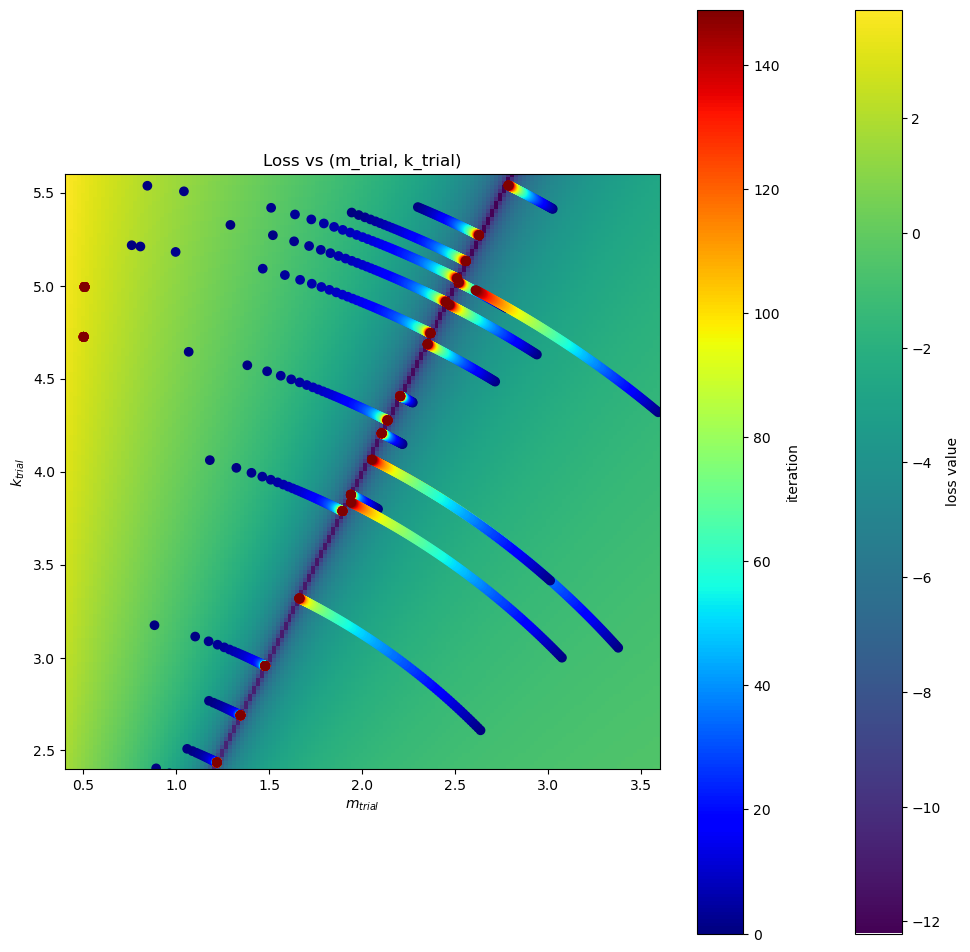
\includegraphics[scale=0.60]{parameter-paths.png}
		\label{fig:parameter-paths}
	\end{figure}
\end{appendices}



\newpage
\begin{appendices}
	\section{Bibliography}
	\printbibliography
\end{appendices}

\end{document}